
\iflong

\else



\begin{frame}
	\frametitle{Learning which Features are Useful}

	\begin{itemize}
		\item Use how humans these data as a prior for supervised maxent model~\cite{daume-04}
		\item Prior for label $a$ and feature $f$ is a function of the number of buzzes $b$ and tf-idf~\cite{salton-68}
\begin{equation}
  \left[ \vphantom{\frac{a}{b}}\alpha \alert<4>{\ind{ b(a,f) > 0}} + \beta \alert<3>{ b(a,f)} + \gamma
  \right] \alert<2>{\mbox{tf-idf}(a,f)} .
\label{eq:meanweight}
\end{equation}
		\begin{itemize}
			\item $\alpha$, $\beta$, and $\gamma = 0$: na\"ive zero prior
			\item $\alpha$ and $\beta = 0$: linear transformation of the mean
			\item $\alpha$ and $\gamma = 0$: number of buzzes times tf-idf value of the features
		\end{itemize}

	\end{itemize}

\end{frame}

\begin{frame}
	\frametitle{Using buzzes as a prior}

\begin{equation*}
  \left[ \vphantom{\frac{a}{b}}\alpha \ind{ b(a,f) > 0} + \beta b(a,f) + \gamma
  \right] \mbox{tf-idf}(a,f) .
\end{equation*}

\begin{center}
\begin{tabular}{cccccc}
Answers & Weighting & $\alpha$ & $\beta$ & $\gamma$ & Error\footnote{Buzz and tf-idf computed on training data; grid search on dev data; error on test data} \\
\hline
\multirow{5}{*}{100} & zero & - & - & - & 0.22 \\
& tf-idf & - & - & 8.3 & 0.08 \\
&  buzz-binary & 10.7 & - & - & {\bf 0.06} \\
&  buzz-linear & - &  1.1 & - & 0.10 \\
& buzz-tier & - & 1.6 & 0.5 & 0.07 \\
\hline
\end{tabular}
\end{center}
\end{frame}




\begin{frame}[t]
	\frametitle{Race Against the Machine}
	\begin{center}

\begin{tabular}{|ll|ccc|c|}
\hline
      &   & \multicolumn{3}{c|}{Human Scoring} & \\
Strategy&	Features & \alert<1>{Average} &	\alert<2>{Best}&	\alert<3>{Median} &	Token\\
\hline
\multirow{4}{*}{Classify}
& text & -8.72 & -10.04 & -6.50 & 40.36 \\
& +guess & -5.71 & -8.40 & -3.95 & 66.02 \\
& +pos & -4.13 & -7.56 & -2.70 & 67.97 \\
& \alert<5>{+change} & {\bf -4.02} & {\bf -7.41} & {\bf -2.63} & 77.33 \\
\hline
\alert<6>{Oracle} &  & 3.36 & 0.61 & 4.35 & 49.90 \\
\hline
                      & \alert<7>{all}             & -6.61         & -9.03         & -4.42 & 100.19 \\
                     & \alert<8>{ftp}              & -5.22         & -8.62         & -4.23 & 88.65 \\
Rapacious             &  \alert<9>{index$_{30}$}   & -7.89         & -8.71         & -6.41 & 32.23 \\
Baseline         &  \alert<9>{index$_{60}$ }       & -5.16         & {\bf -7.56}   & -3.71 & 61.90 \\
                      & \alert<9>{ index$_{90}$ }  & {\bf -5.02}   & -8.62         & {\bf -3.50} & 87.13 \\
\hline
\end{tabular}
	\end{center}
\vspace{-1cm}
% \only<4>{ \paragraph{token} Where the algorithm buzzed in.}
\only<6>{ \paragraph{Oracle} Best possible incremental strategy \emph{post hoc}}
\only<5>{ \paragraph{Classify} Incremental algorithms doing best, but not that well}
\only<7>{ \paragraph{all} This strategy waits until the end of the question and answers the best
  answer possible.}
\only<8>{ \paragraph{ftp} Waiting until when ``for 10 points'' is said, then giving the
    best answer possible.}
\only<9>{ \paragraph{index-n} Waiting until the first feature after the $n^{th}$ token has been processed, then giving the best answer possible.  }
\only<1> { \paragraph{average} For each human who answered a question, compare the positions and compute a reward.  Average them.}
\only<2> { \paragraph{best} For each question, take the human buzz position to be the the
  earliest that \emph{any} human buzzed in the question}
\only<3> { \paragraph{median} For each question, take the human buzz position to be the
  earliest position after 50\% of human buzzes appeared.}
\end{frame}


\begin{frame}{Richer Content Models}

\begin{enumerate*}
  \item For each category $c$ of questions, draw a distribution over words
    \alert<4>{$\theta_c \sim \dir{\lambda_1 \theta_0}$}.
    \begin{itemize*}
   \alert<3>{ \item For each label $l$ in category $c$, draw a distribution over words
      $\theta_{l,c} \sim \dir{\lambda_2 \theta_c}$ }
   \alert<2>{   \item For each type $v$, draw a bigram distribution $\theta_{l,c,v} \sim
        \dir{\lambda_3 \theta_{l,c}}$ }
  \end{itemize*}
  \item Draw a distribution over labels $\phi \sim \dir{\alpha}$.
  \item For each question with category $c$ and $N$ words, draw answer $l \sim \mult{\phi}$:
    \begin{itemize*}
\footnotesize
      \item Assume $w_0 \equiv \mbox{\textsc{Start}}$
     \alert<1>{ \item Draw $w_n \sim \mult{\theta_{l,c,w_{n-1}}}$ for $n \in \{1 \dots N\}$ }
    \end{itemize*}
\end{enumerate*}

\only<5>{
 
\vspace{-4cm}

  \begin{block}{Short story:}
    \begin{itemize}
      \item Models know universe of possible categories ({\bf cat}),
    \item How questions were structured ({\bf
      bigram})
    \item Will hopefully do better than ({\bf na\"ive}) model
      \end{itemize}
    \end{block}
}

\end{frame}

\begin{frame}[t]

\frametitle{Error Analysis}

\begin{columns}

	\column{.4 \linewidth}
        \only<5-> {

		\begin{itemize}
			\item \alert<5> { Too slow }
			\item \alert<6> {Coreference \cite{haghighi-07} and correct question
type \cite{moldovan-00}}
			\item \alert<7> {Not enough information / not weighting later clues higher }
		\end{itemize}

}

	\column{.6 \linewidth}

		\begin{center}
			\only<1>{  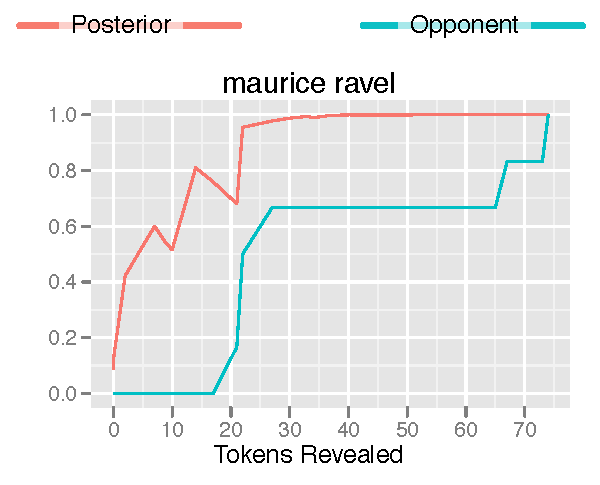
\includegraphics[width=.9\linewidth]{qb/real_question_ravel_0} \\ }
			\only<2>{  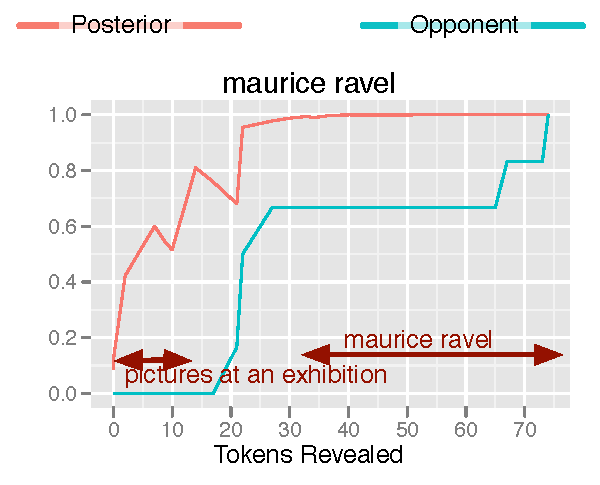
\includegraphics[width=.9\linewidth]{qb/real_question_ravel_1} \\ }
			\only<3>{  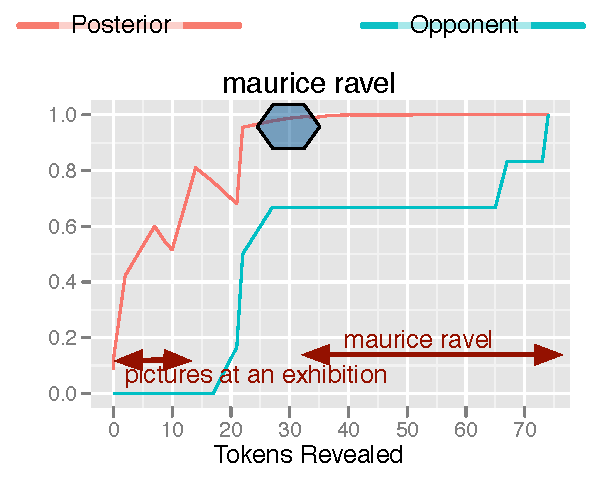
\includegraphics[width=.9\linewidth]{qb/real_question_ravel_2}
                          \\ }
			\only<4-5>{  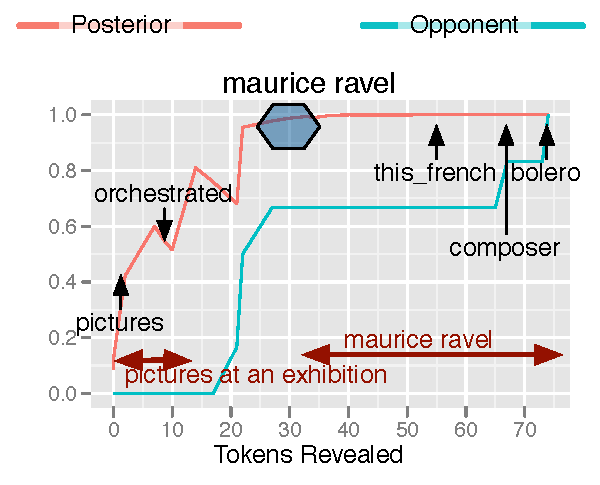
\includegraphics[width=.9\linewidth]{qb/real_question_ravel_3} \\ }
			\only<6>{  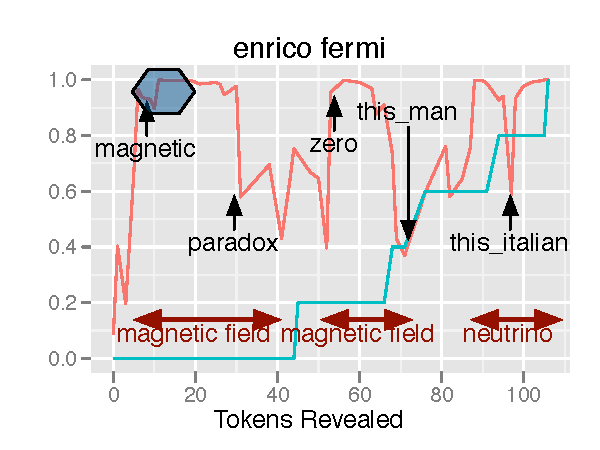
\includegraphics[width=.9\linewidth]{qb/real_question_fermi} \\ }
			\only<7>{  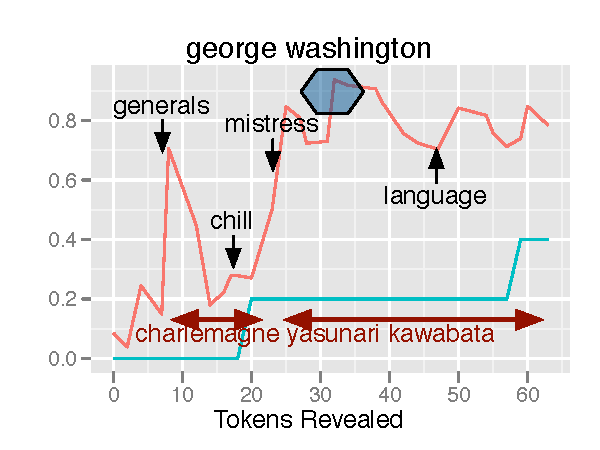
\includegraphics[width=.9\linewidth]{qb/real_question_washington} \\ }
			\only<2>{ 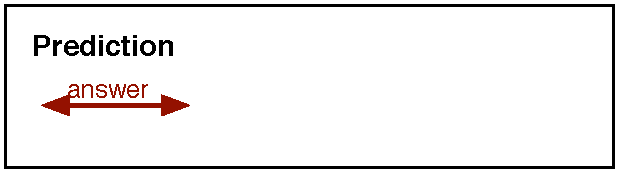
\includegraphics[width=.9\linewidth]{qb/real_question_key_0} }
			\only<3>{ 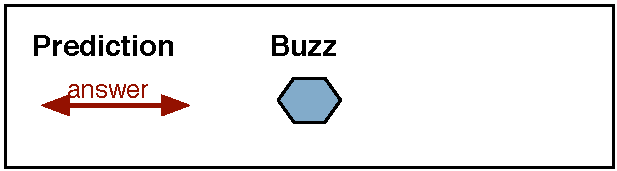
\includegraphics[width=.9\linewidth]{qb/real_question_key_1} }
			\only<4->{ 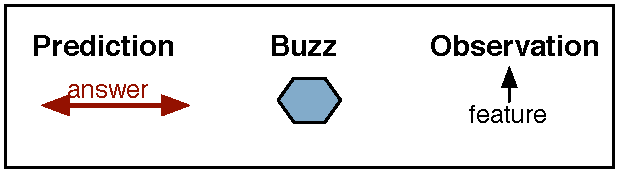
\includegraphics[width=.9\linewidth]{qb/real_question_key_2} }
		\end{center}
\end{columns}

\end{frame}


\fi


\begin{frame}

\frametitle{Logistic Regression}

\begin{tabular}{rrrrr}
  \hline
 & Estimate & Std. Error & z value & Pr($>$$|$z$|$) \\
  \hline
(Intercept) & -2.6200 & 0.0368 & -71.10 & 0.0000 \\
  Tokens revealed & 0.0229 & 0.0001 & 214.00 & 0.0000 \\
  ``ftp'' seen & 0.6677 & 0.0083 & 80.73 & 0.0000 \\
  Years after 2000 & -0.0005 & 0.0000 & -11.53 & 0.0000 \\
  Biology & -0.8975 & 0.0417 & -21.52 & 0.0000 \\
  Chemistry & -0.0323 & 0.0398 & -0.81 & 0.4171 \\
  Earth Science & -0.5980 & 0.1085 & -5.51 & 0.0000 \\
  Fine Arts & -0.6800 & 0.0372 & -18.29 & 0.0000 \\
  History & -0.5083 & 0.0374 & -13.61 & 0.0000 \\
  Literature & -0.6133 & 0.0368 & -16.65 & 0.0000 \\
  Mathematics & -0.5810 & 0.0530 & -10.95 & 0.0000 \\
  Other & -1.2591 & 0.0773 & -16.29 & 0.0000 \\
  Physics & -0.7292 & 0.0405 & -18.02 & 0.0000 \\
  Social Studies & -0.5607 & 0.0369 & -15.18 & 0.0000 \\
   \hline
\end{tabular}

\end{frame}

\begin{frame}
	\frametitle{Incremental Classification}
	\begin{block}{When to buzz?}
	\begin{equation}
  \mbox{Q}(X_n^{\mbox{new}}) =  \mbox{R}  \left(X_n^{\mbox{old}}\right) -
  \mbox{R}\left(X_n^{\mbox{old}} \cup
  X_n^{\mbox{new}}\right) - \mbox{\textsc{Waiting-Cost}}\left(X_n^{\mbox {new}}\right),
\label{eq:util}
\end{equation}
where the R is the expected reward given your best guess $\mbox{MC-Cost}(X_n) = $
\begin{equation*}
\alert<2>{\e{X_n}{ \max_{i} \rho p(z_n = i | X) + \sum_{j \not = i} \omega p(z_n = j | X)  }},
\end{equation*}
	\end{block}

\end{frame}